\documentclass{llncs}
% Grundgröße 12pt, zweiseitig
% Standardpakete
% richtiges encoding fuer verschiedene compiler
\usepackage{iftex}
\ifPDFTeX
   \usepackage[utf8]{inputenc}
   \usepackage[T1]{fontenc}
   \usepackage{lmodern}
\else
   \ifXeTeX
     \usepackage{fontspec}
   \else 
     \usepackage{luatextra}
   \fi
   \defaultfontfeatures{Ligatures=TeX}
\fi
% deutsche Silbentrennung
\usepackage[english]{babel}
\usepackage{amsmath}
\usepackage{cite}
\usepackage{float}
\usepackage{subfig}

% Grafiken einbinden
\usepackage{graphicx}
\graphicspath{{figures/}}

\usepackage{hyperref}
% tiefe des Inhaltsverzeichnisses
\setcounter{tocdepth}{2}


\begin{document}

\title{Project proposal: Comparative exploration of old and modern AI Methods with Abalone}
\author{Ture Claußen, 202132027, \email{ture.claussen@stud.hs-hannover.de}}
\authorrunning{T. Claußen}
\institute{Dept. of Software and Computer Engineering, Ajou University}

% jetzt gehts los
{\def\addcontentsline#1#2#3{}\maketitle} % Wird gebraucht, damit der Title nicht im Inhaltsverzeichnis steht

\begin{abstract}
  Games provide the perfect environment for artificial agents to navigate in. Especially for the
  \keywords{AI \and Alpha-beta \and Q-Learning \and Abalone \and Intelligent Agents}
\end{abstract}

\section{Introduction}

Abalone is a fairly new game, that was devised in 1987 by Michel Lalet and Laurent Lévi \cite{noauthor_abalone_2020}. It is a two-player game consisting of a hexagonal board with 61 fields and 14 marbles for black and white respectively. The goal of the game is to push six of the opponent's marbles of the playing field.

\subsection{Rules}

\begin{figure}[!h]
  \centering
  \subfloat["In-line" moves]{
    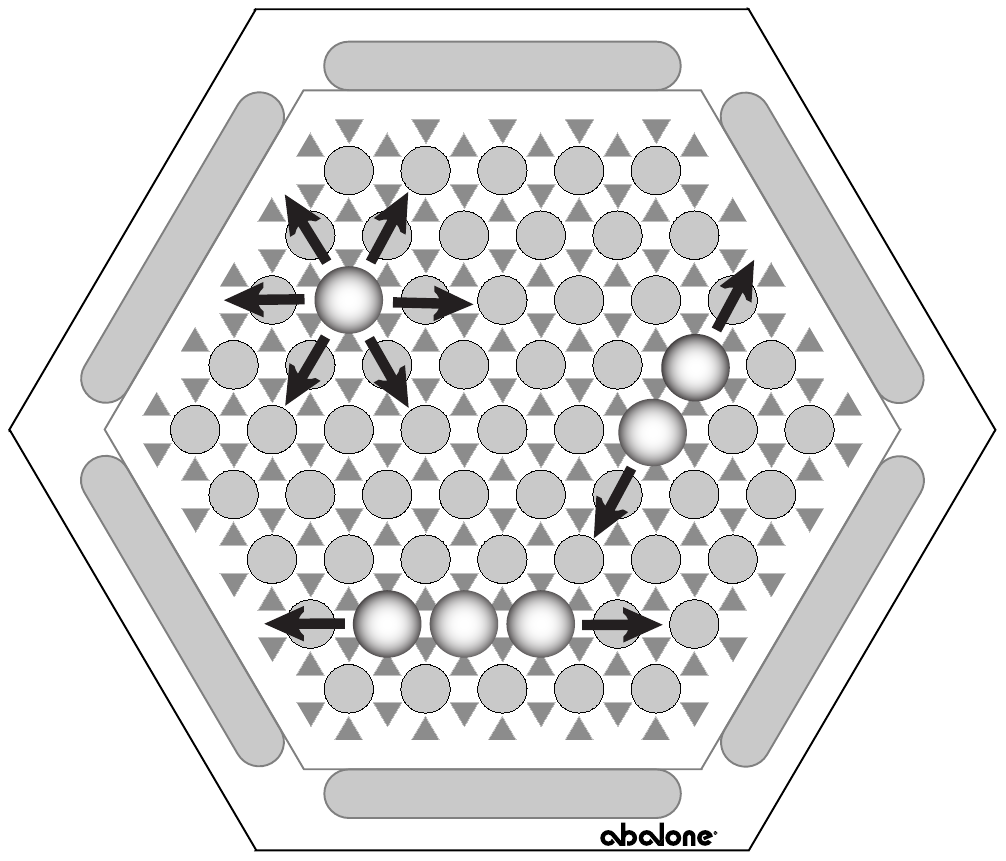
\includegraphics[width=5cm, keepaspectratio]{rules_inline_move.png}
  }
  \hfill
  \subfloat["Side-step" moves]{
    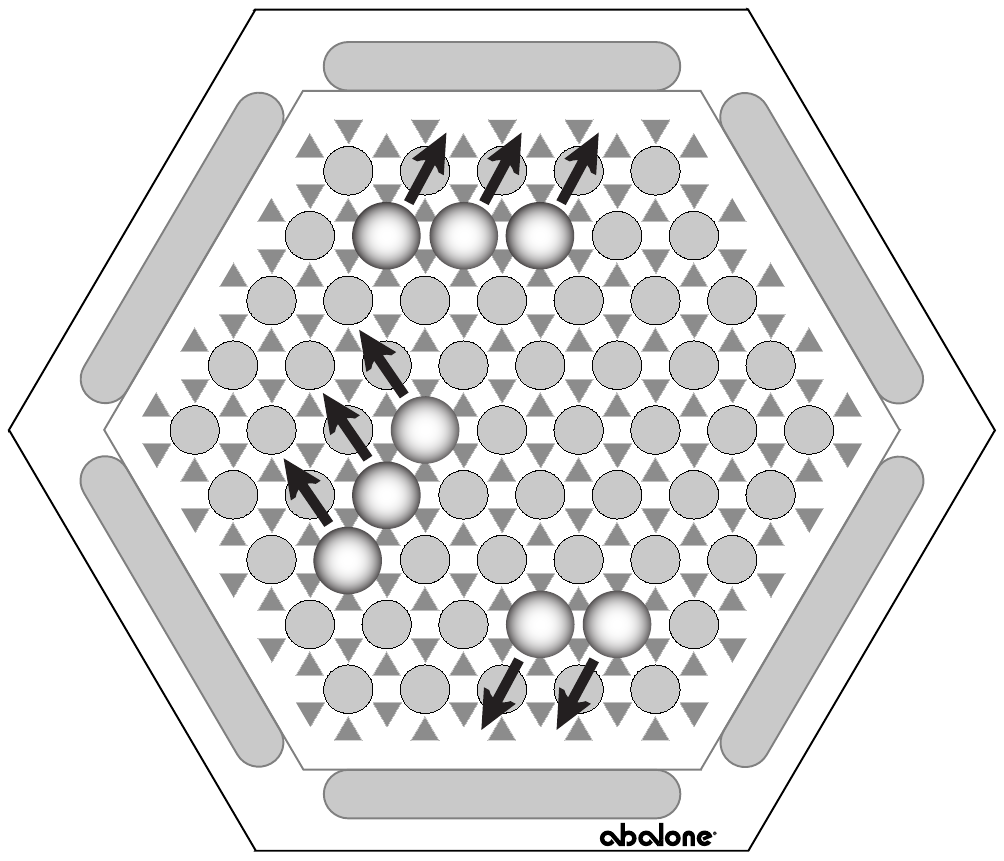
\includegraphics[width=5cm, keepaspectratio]{rules_side_step_move.png}
  }
  \caption{Basic moves \cite{abalone_sa_abalone_nodate}}
\end{figure}

\begin{figure}[!h]
  \centering
  \subfloat["2-push-1" sumito]{
    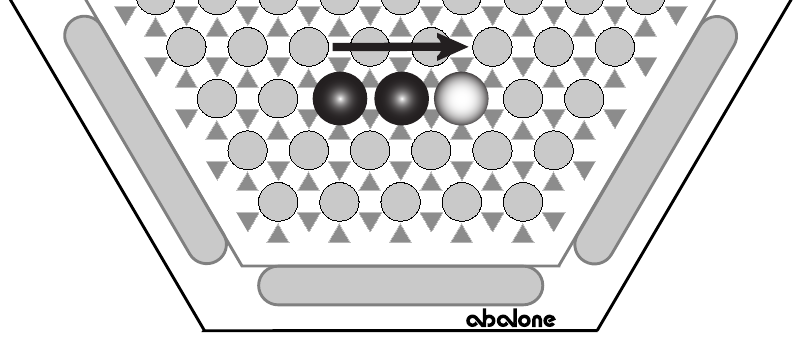
\includegraphics[width=3cm, keepaspectratio]{rules_2-push-1_sumito.png}
  }
  \hfill
  \subfloat["3-push-1" sumito]{
    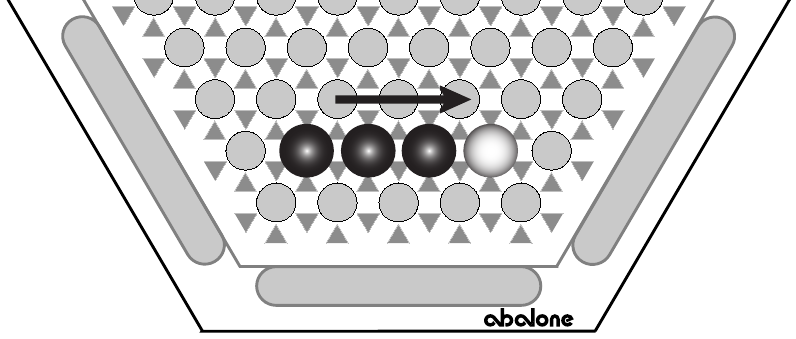
\includegraphics[width=3cm, keepaspectratio]{rules_3-push-1_sumito.png}
  }
  \hfill
  \subfloat["3-push-2" sumito]{
    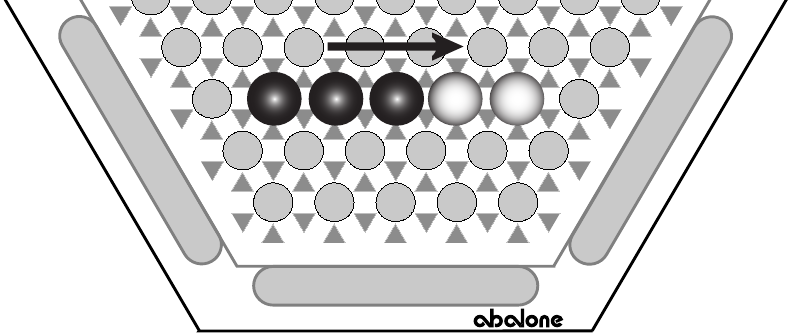
\includegraphics[width=3cm, keepaspectratio]{rules_3-push-2_sumito.png}
  }
  \caption{Sumito positions allow pushing the opponents marbles \cite{abalone_sa_abalone_nodate}}
\end{figure}

\subsection{Complexity}

\paragraph{State space complexity}

$$
  \sum_{k=8}^{14}\sum_{m=9}^{14}\frac{61!}{k!(61-k)!}\times\frac{(61-k)!}{m!((61-k)-m)!}
$$

\paragraph{Game tree complexity}

\paragraph{Comparative complexity}

\section{Project details}

\subsection{Agent design}

Based on the PEAS framework we can analyze the task environment for the agent. \cite[p.107]{russell_artificial_2021}

\begin{description}
  \item[Performance measure] Win/loss, number of moves, time to deliberate
  \item[Environment] Digital playing board
  \item[Actuators] Move marbles, display text to CLI
  \item[Sensors] Position of marbles
\end{description}



\subsection{Algorithm comparision}

\subsection{}

\section{Conclusion}

% Literatur
\bibliographystyle{splncs04.bst}
\bibliography{ref.bib}
\end{document}